\documentclass[12pt, preprint]{aastex}

% words
\newcommand{\project}[1]{\textsl{#1}}
\newcommand{\documentname}{\textsl{Article}}
\usepackage{color}
\bibliographystyle{apj}

\usepackage{hyperref}
\newcommand{\niceurl}[1]{\href{#1}{\textsl{#1}}}


% To-do:
%  - do we get the same result with the official WISE coadds (vs unWISE)?
%  -> viewer in L,B ?
%  - Galactic L,B grid lines?
%  - ensure that Figure 1 galactic L,B are labelled correctly!  Is the LMC in the right place?

% @melissakness:
% -- must check in Xbulge_bib!
% -- are the |\ell|s ok?
% -- is it worth saying what the exponential disk model fit parameters are
%    in physical units?

% @dstndstn:
%  - Makefile
%  - clean up, fully document, and add comments pointing to the 
%    figure-generating code
%  - redo the unWISE coadds using the same code as the AllWISE ones
%  - redo the unWISE coadds using Aaron's new ones?
%  - cite AllWISE release (search ``official'')



\newcommand{\viewerurl}{\niceurl{http://legacysurvey.org/viewer}}

\begin{document}

\title{The X-shaped Bulge of the Milky Way revealed by WISE}
\author{%
Melissa Ness\altaffilmark{1,2} \& %\and
Dustin Lang\altaffilmark{3,4}
}
%
\shortauthors{Ness, Lang}
\altaffiltext{1}{%
  Max-Planck-Institut f\"ur Astronomie,
  K\"onigstuhl 17, D-69117 Heidelberg, Germany
}
\altaffiltext{2}{%
  To whom correspondence should be addressed:
  ness@mpia-hd.mpg.de
}
\altaffiltext{3}{%
  Dunlap Institute and Department of Astronomy \& Astrophysics,
  University of Toronto,
  50 Saint George Street, Toronto, ON, M5S 3H4, Canada
}
\altaffiltext{4}{%
  Department of Physics \& Astronomy,
  University of Waterloo,
  200 University Avenue West, Waterloo, ON, N2L 3G1, Canada
}
% the X-shaped morphology is believed to be tied to % generic formation history of nearby spiral galaxies 
\begin{abstract}%
The Milky Way bulge has a boxy/peanut morphology and an X-shaped structure. This X-shape has been revealed by the `split in the red clump' from 
star counts along the line of sight toward the bulge, measured from photometric surveys. This boxy, X-shaped bulge morphology is not unique to the Milky Way and such bulges are observed in other barred spiral galaxies.  N-body simulations show that boxy and X-shaped bulges are formed from the disk via dynamical instabilities.  It has also been proposed that the Milky Way bulge is not X-shaped, but rather, the apparent split in the red clump stars is a consequence of different stellar populations, in an old classical spheroidal bulge. We present a WISE image of the Milky Way bulge, produced by downsampling the publicly available ``unWISE'' coadds. The WISE image of the Milky Way bulge shows that the X-shaped nature of the Milky Way bulge is self-evident and irrefutable. The X-shape morphology of the bulge in itself and the fraction of bulge stars that comprise orbits within this structure has important implications for the formation history of the Milky Way, and, given the ubiquity of boxy X-shaped bulges, spiral galaxies in general. 
\end{abstract}



\keywords{%
}

\section{Introduction}\label{sec:Intro}

The boxy nature of the bulge of the Milky Way was first revealed in the COBE satellite image \citep{Dwek1995}. Using photometric data from the VVV survey, \citet{Wegg2013} measured the three dimensional density of red clump stars in the bulge, earlier revealed to show two peaks along the line of sight \citep{McWilliam2010, Nataf2010}, and determined their distribution to be characteristic of a strong boxy/peanut bulge within a barred galaxy. This observed split in the red clump is reported to be a property of the more metal rich stars in the bulge, with [Fe/H] $>$ --0.5 \citep{Ness2012, Uttenthaler2012}; although according to \citet{Nataf2014} this metallicity dependence may be subject to biases.  \citet{Portail2015b} used the VVV red clump stellar density to show that the Milky Way's bulge has an off-centered X-structure and using constraints from kinematic data, determined that the fraction of stars in orbits that contribute to the X-shape is 40--45\% of the mass of the bulge \citep{Portail2015a}. The X-shape in the Milky Way bulge is similar to that seen in the unsharp masked images of other barred spiral galaxies  \citep[e.g.][]{Bureau2006}. Such X-shaped structures, which underly the boxy/peanut, have been shown to form in N-body simulations, via dynamical instabilities in the disk \citep[e.g.][]{Athanassoula2005, Debattista2006, Inma2006}. This shape is a consequence of the x$_{1}$v$_{1}$ \citep{P1984, Athanassoula1992} and other orbit families \citep[e.g.][]{Portail2015b}. 

\citet{Lee2015} have questioned the existence of the X-shaped nature of the bulge, instead proposing the split in the red clump stars to be a consequence of different stellar populations in a classical bulge. Conversely,  \citet{Gonzalez2015} summarise the set of observational properties of the bulge which explain the link between the double or split red clump and the X-shape.


 We present, for the first time, the WISE image of the Milky Way \citep{Lang2014a} which clearly demonstrates the Milky Way bulge is irrefutably morphologically, X-shaped. This follows expectations from the observational evidence,  from dynamical models of boxy/peanut bulges like the Milky Way, and from observations of other barred galaxies that reveal such an X-shaped profile is not uncommon \citep{L2014}. 

\section{The unWISE image of the Milky Way bulge}

The Wide-Field Infrared Survey Explorer (WISE, \citet{W2010}) is a full sky photometric survey using four bands in the mid-infrared at 3.4 $\micron$, 4.6 $\micron$, 12 $\micron$ and 22 $\micron$ (W1--W4). The original WISE data release was based on a co-adding approach that is optimal for detecting isolated point sources but which effectively blurs the images. \citet{Lang2014b} implemented an alternative co-adding methodology that does not degrade the resolution of the imaging.  These ``unWISE'' coadds have been publicly released.\footnote{Available at \niceurl{http://unwise.me}}

Figure \ref{fig:xbulge} presents the bulge region of the Milky Way,  resampled to galactic coordinates from the unWISE images from \citet{Lang2014a} \footnote{Also available in interactive RA,Dec coordinates at \viewerurl}, across $(|\ell|,|b|)$ $<$ (60, 30).  This image shows WISE bands W1 and W2. This presents the overall Milky Way structures in exquisite detail.
No additional unsharp masking or equivalent techniques have been used to enhance these data. The bulge in the central region of this Figure shows a clear X-shaped morphology. Note that the arms of the X-shape are asymmetrical around the minor axis and appear larger at left than at right. This is a real projection effect and reflects that the bulge is oriented at about 27$^\circ$ degrees with respect to the line of sight \citep{Wegg2013}, with the nearest side at positive longitudes. The X-shape is also visible, though with more artifacts, in the official AllWISE data release imaging.

%Using the W3 and W4 images from the AllWISE data, it is difficult to see the X-shape structure due to variation in the background levels. 

\begin{figure}[h!]
\centering
        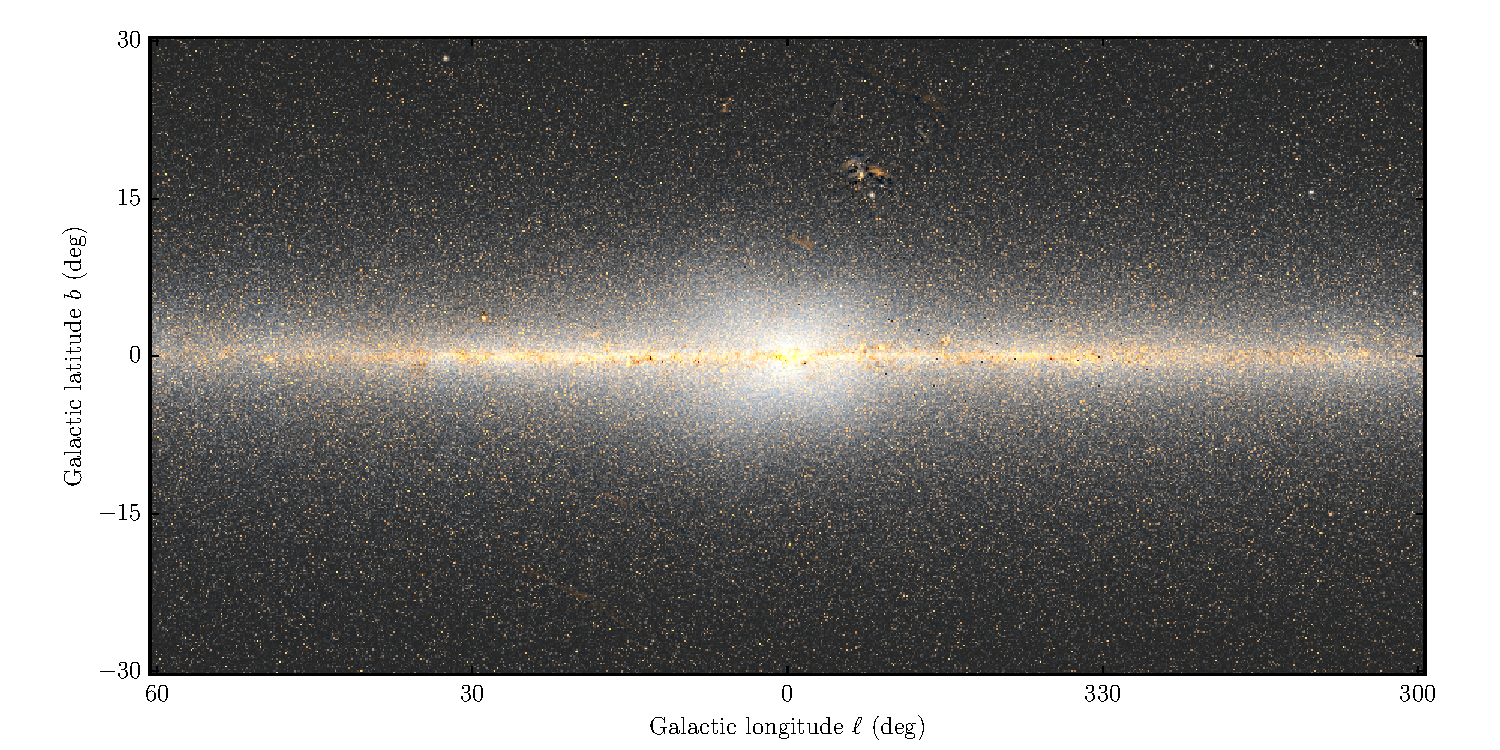
\includegraphics[width=\textwidth]{xbulge-00}
\caption{WISE image for W1 and W2 in Galactic coordinates.  An arcsinh
  stretch is used to allow the full dynamic range to be shown.}
% and put link to webpage where this is: \viewerurl}
\label{fig:xbulge}
\end{figure}

\section{The contrast enhanced unWISE image of the bulge}

Figure \ref{fig:filt} presents a contrast enhanced and zoomed in version of Figure \ref{fig:xbulge}. This better reveals the X-shape light profile of the bulge and its extent across $(\ell,b)$ in the WISE image. This Figure was produced with a median subtraction across each row to suppress the contribution from the disk. The arms in the image extend to longitudes of $\ell$ $\approx$ 10$^\circ$ and latitudes of $|b|$ $\lesssim$ 10$^\circ$; (although note again the arms on the near side are larger than those of the far side due to projection). This extent on the sky corresponds to a length of about 2.4 kpc for each arm, for a distance of the bulge of 8.3 kpc from the Sun and a bar angle of 27$^\circ$.

\begin{figure}[h!]
\centering
        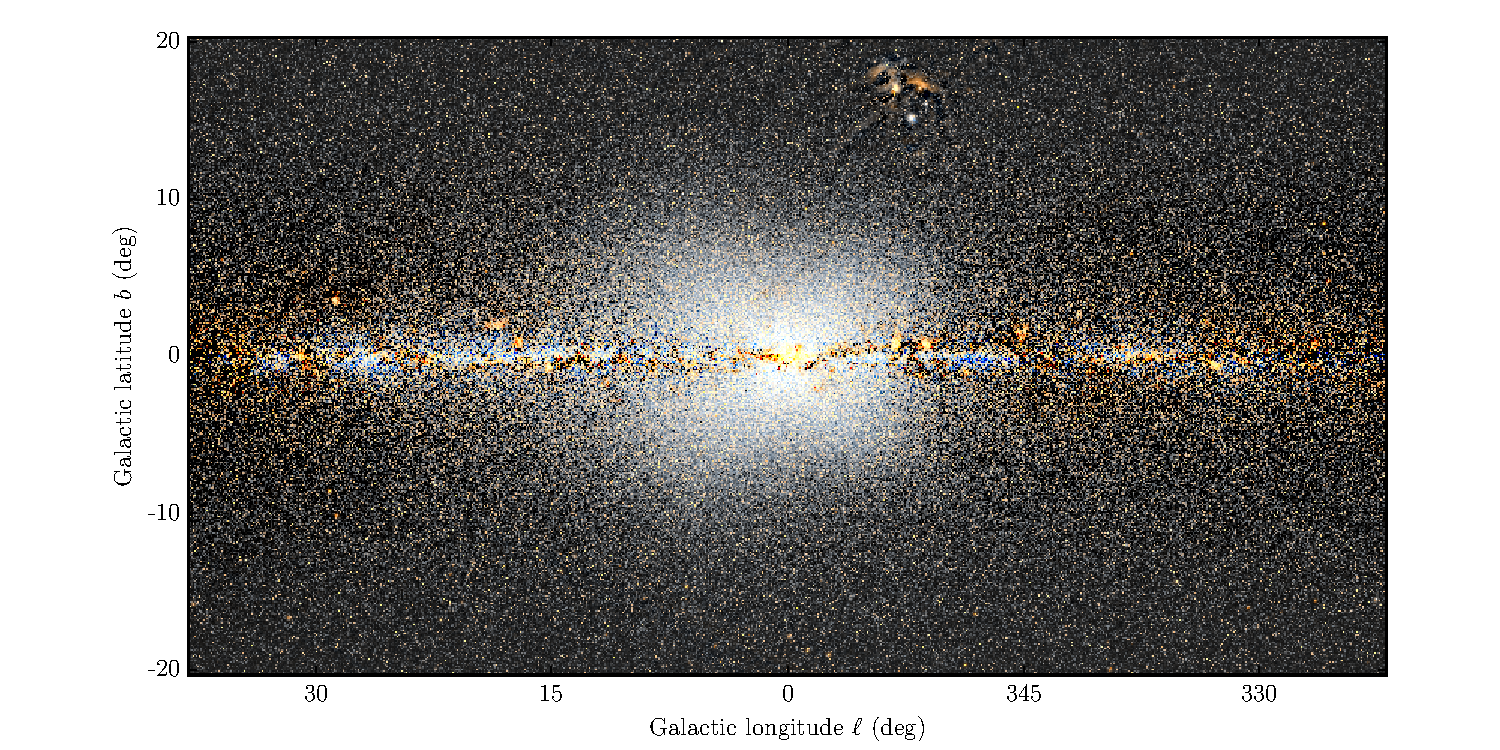
\includegraphics[width=\textwidth]{xbulge-01}
\caption{The same as Figure 1, but zoomed in and with the median of each row of the image subtracted to provide a better contrast which reveals the X-shape morphology in better detail.}
\label{fig:filt}
\end{figure}

\section{The residuals of the unWISE image of the bulge}

Finally, we fit and subtract a simple exponential disk model to make the bulge structure more clear.  We zoom in to the central region of the galaxy, compute the W1 - W2 color of each pixel, and mask the top and bottom 5\% in order to largely suppress the most dusty regions.  We then fit a simple exponential disk model, where the shape parameteres are shared between the W1 and W2 bands, and each pixel is given equal weight.
Figure \ref{fig:modfit} shows these results.
The two left hand panels show the data and model, respectively (both masked). The residuals are shown in the top right hand panel of Figure \ref{fig:modfit} and the 40-pixel median of this residual is shown in the bottom left panel. The regions of excess dust above the masked panel in the plane show some of the (dark)  regions of dusty lanes at the galactic centre (e.g. across (--5$^\circ$ $<$ $l$ $<$ 8$^\circ$, $|b|$ $<$ 2$^\circ$). The white regions show the stellar excess above the exponential disk.
%The bottom right panel of Figure \ref{fig:modfit} shows the outliers in the residual image at top right masked by a blue color mask, keeping the 5th to 95th percentile of the W1-W2 color.
The projection effect is again clear in these residual maps, which reflects that the bulge is orientated at 27$^\circ$ with respect to the line of sight, with the nearest side at  positive longitudes. %
%The arms of the X at left in the bottom panel of Figure \ref{fig:modfit} trace out an off-centre X-structure, as revealed in\citep{Portail2015b}. 

\begin{figure}[h!]
\centering
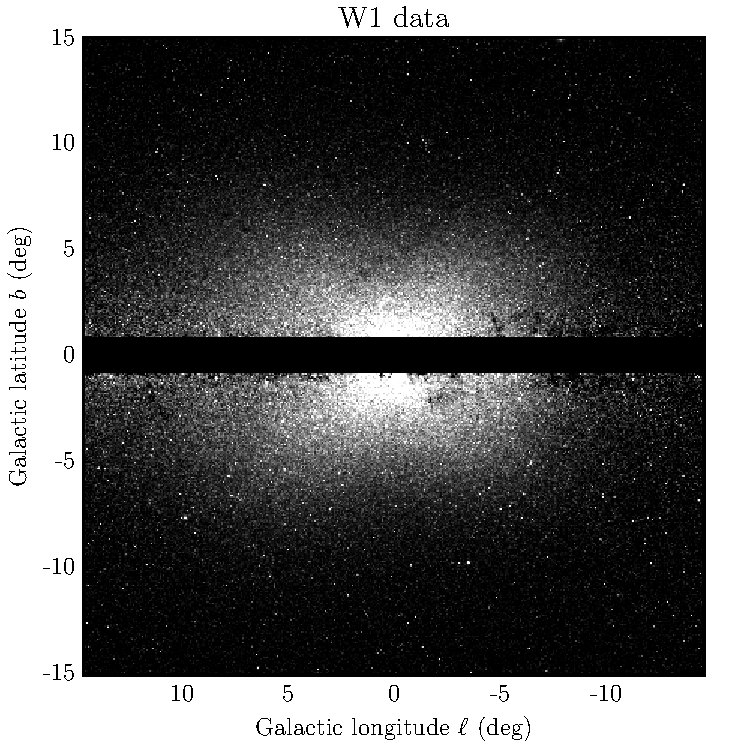
\includegraphics[width=0.3\textwidth]{xbulge-04}
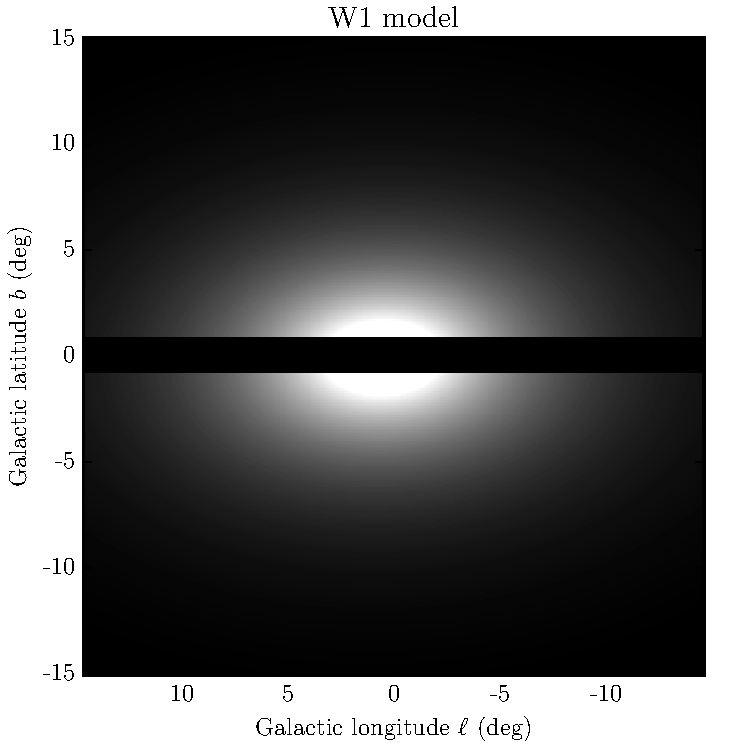
\includegraphics[width=0.3\textwidth]{xbulge-08}
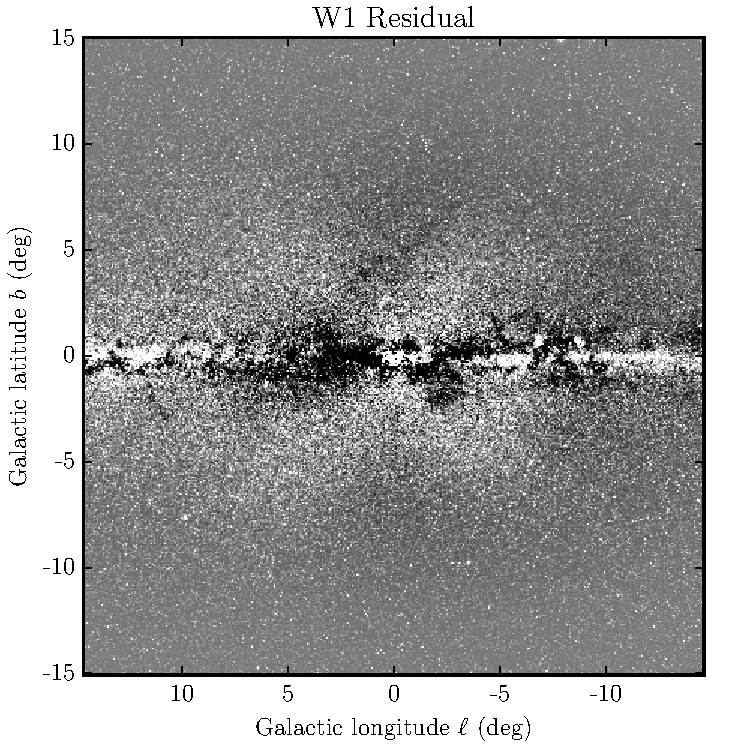
\includegraphics[width=0.3\textwidth]{xbulge-09}
\\
\rule{0.3\textwidth}{0pt}
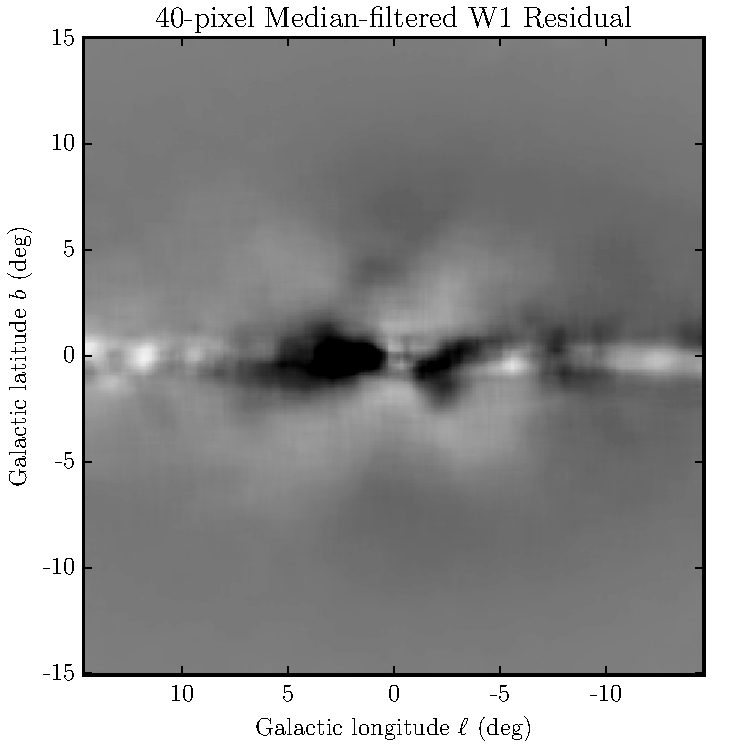
\includegraphics[width=0.3\textwidth]{xbulge-10}
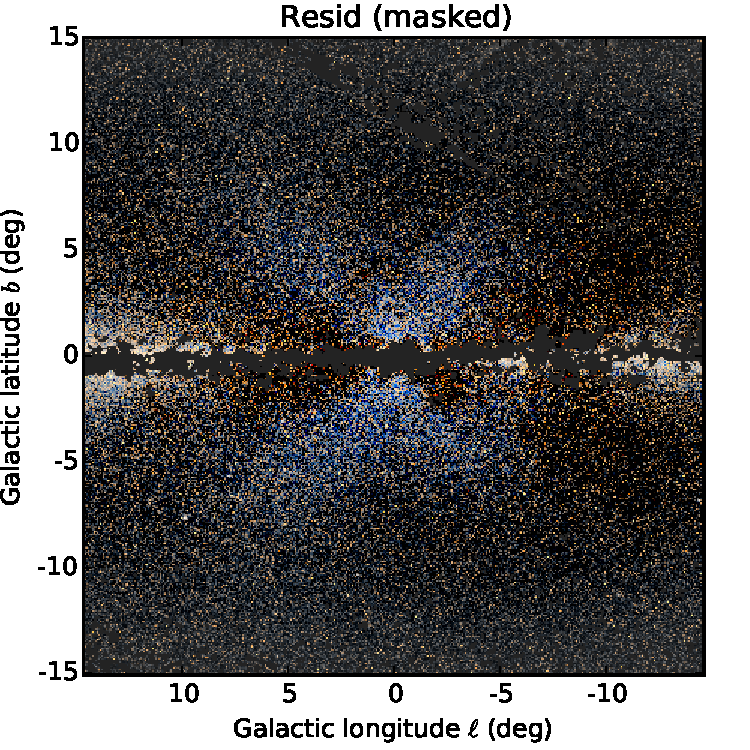
\includegraphics[width=0.3\textwidth]{xbulge-12}
\caption{The WISE W1 image fit by a simple exponential disk model, masking
  out the core of the Galactic plane.  In the residuals, the X
  structure becomes more apparent, and is clear in the masking outliers by colour done in the bottom right panel.}
\label{fig:modfit}
\end{figure}




\section{Conclusion}

Using the publicly avilable ``unWISE'' coadds, which implement a new technique that does not degrade the resolution of the imaging, we have presented new images of the bulge of the Milky Way. These directly reveal its X-shaped nature in the integrated light, even without any special image processing or enhancement. Our contrast enhancement and residual maps of the W1 band further highlight the extent of the X-shape that underlies the boxy structure. Critical to understanding the bulge is a further and detailed characterisation of the stars that are in the arms of the X-shape, the spatial extent of which is clearly demonstrated in our Figures. The spatial mapping we have presented in galactic coordinates will therefore provide a useful guide for current and future spectroscopic surveys such as APOGEE \citep{Majewski2015}, 4-MOST \citep{4most} and bulge programs associated with the GALAH survey \citep{deSilva2015}. These data can be used to guide stellar target selection, where examining the spectroscopic ages \citep[e.g.][]{Martig2016, Ness2016} and metallicities of stars in the arms of the X-shape as a function of (l,b) will be necessary to understand the formation of the bulge and constrain the formation processes relevant in the Milky Way. 


\section{Acknowledgements} 
We thank Hans-Walter Rix (MPIA) for helpful comments on this work. 
The research has received funding from the European Research Council under the European Union's Seventh Framework Programme (FP 7) ERC Grant Agreement n.~[321035].
%
The Dunlap Institute is funded through an endowment established by the David Dunlap family and the University of Toronto.

\bibliography{Xbulge_bib.bib}

\end{document}

\begin{figure}
\centering
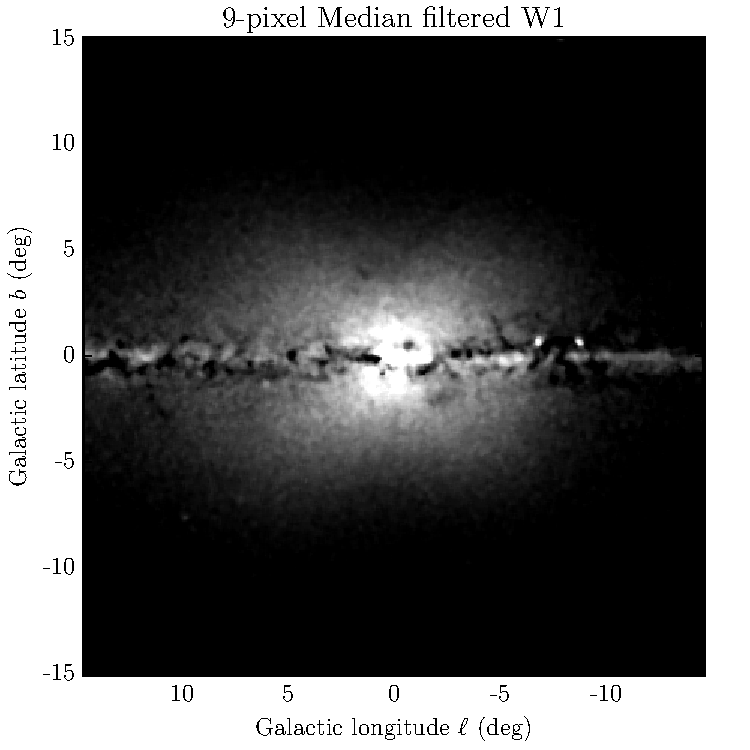
\includegraphics[width=0.3\textwidth]{xbulge-05}
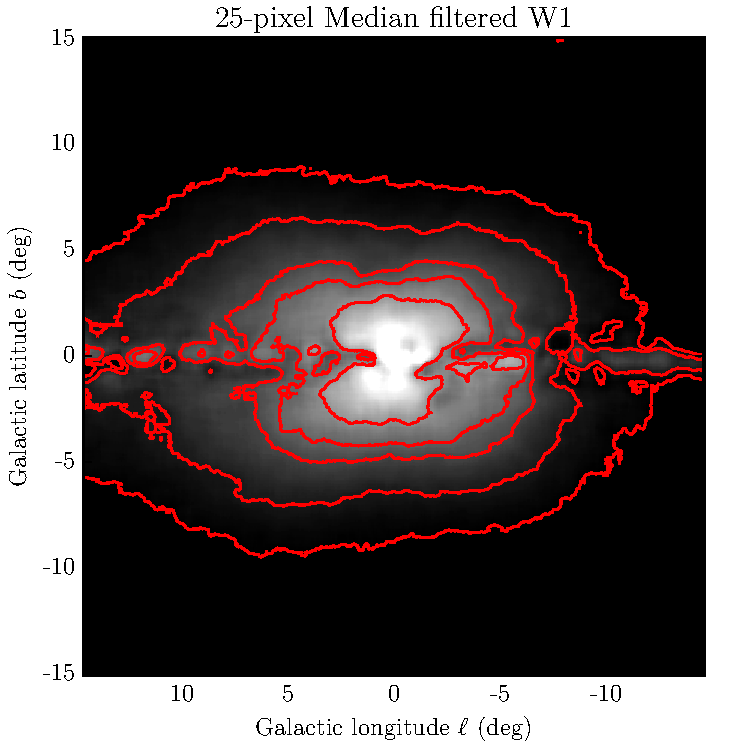
\includegraphics[width=0.3\textwidth]{xbulge-07}
\caption{
}
\label{fig:contours}
\end{figure}


